%% This is an example first chapter.  You should put chapter/appendix that you
%% write into a separate file, and add a line \include{yourfilename} to
%% main.tex, where `yourfilename.tex' is the name of the chapter/appendix file.
%% You can process specific files by typing their names in at the 
%% \files=
%% prompt when you run the file main.tex through LaTeX.
\chapter{State of the Art}
The problem of human action classification or pedestrian intent prediction from a sequence of images has got huge attention from the researchers in recent years. 
This problem is inherently complex as it is based on other 
complex problems. To detect the action or intention one must first detect the object in an image and classify it. Track the same object over several continuous frames to identify the intention. There are several proposals proposed for person detection, many of them try to achieve high accuracy at the expense of high computational cost. This leads many of such proposal not useful for real time application such driver-less cars.   
Before the dominance of convolutional neural network (CNN) and Deep Learning which has outperformed other traditional methods in the recent times. Several researchers found some interesting and great methods, some such nice work done by researchers in these area shall be presented and discussed in the subsequent sections. In general we can think of two types activity prediction, (i) early activity detection (ii) future activity prediction. In the case of early activity detection, the class label of an action is inferred at the point when the activity starts or shortly after the activity started. Where as in the future activity prediction, the class label of the action that will happen next is predicted and also the starting time in the future is also predicted.
 
\section{DPM model based on Manual feature extraction}
\subsection{HOG }
In year 2005 Dalal \& Triggs found a method which is superior to Haar wavelets descriptor and other state-of-the-art method based on edge and gradient, at that time for the task of pedestrian detection. HOG descriptors are comparable with edge orientation histogram, SIFT \footnote{Scale Invariant Feature Transform, by transforming image data into scale invariant co-ordinates relative to local features \cite{lowe2004distinctive}} descriptors and shape context, however these are computed on a dense grid of uniformly spaced cell and use overlapping local contrast normalization. Which they named as Histograms of Oriented Gradient (HOG) features\cite{dalal2005histograms}. The gradient is computed by applying a filter kernel \\
\begin{center}
$[-1,0,1] \, and \, [-1,0,1] ^{T}$
\end{center}

\newpara After computation of the gradient they are gradient values are used to update a 9 histogram channel which are evenly spread over 0-180 degrees or 0-360 degrees. They tried peson/non-person classification using this robust feature descriptor and Linear SVM and got state-of-the-art result of that time.

\newpara
Pedro F. Felzenszwalb and team proposed deformable part model (DPM) \cite{felzenszwalb2009object} which is based on pictorial structures that represent objects by means of a collection of object parts arranged in a deformable configuration. Each object part captures local appearance properties of
an object and the deformable configuration is identified  by spring-like connections between certain pairs of such parts. They use a variation of Support Vector Machine(SVM) which they named as latent SVM (LSVM) is used for the training of the model and  histogram of oriented gradients (HOG) used for features vector. After the success of usages of CNNs in tasks like image classification, CNNs are used to extract the feature sets instead of manual extraction. CNNs found to be outperform manual feature extraction as they are principally designed Neural net \textbf{architecture which preserves local connections and shares weights}.

\section{CNN based feature extraction}
\newpara  CNN are special type of multilayer perceptrons, based shared weight architecture and inspired by biological connectivity between neurons in human visual cortex. A particular neuron respond to stimuli only in a restricted region of the visual field called receptive field. CNNs employs a special kind of linear operation called convolution. CNN is characterized by several convolution and pooling operation and finally followed by one or more fully connected layers.

\begin{figure}[t!]
	\centering
	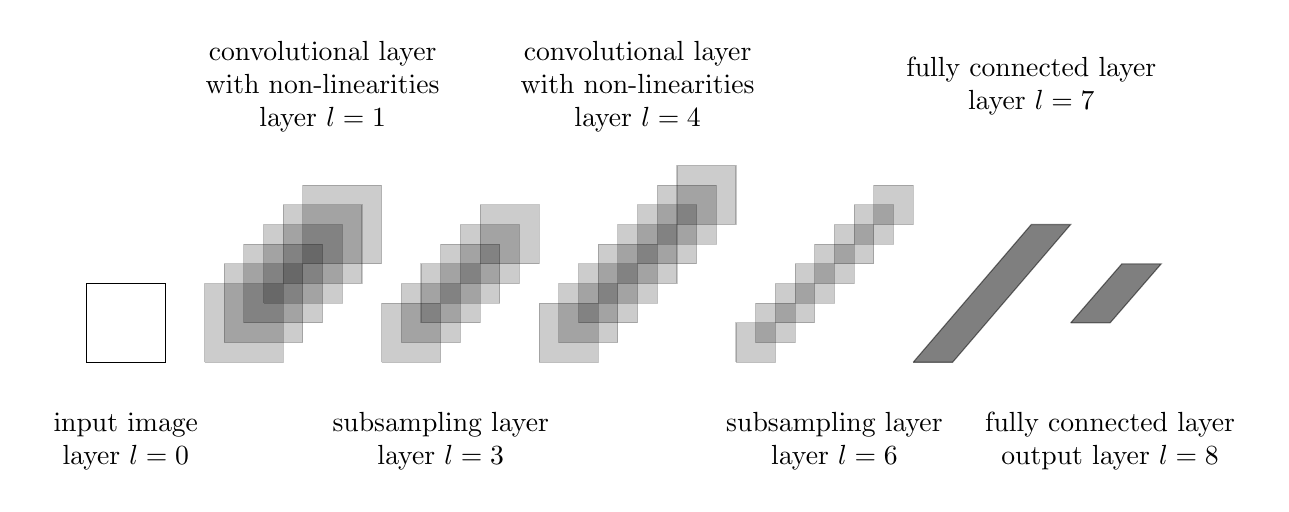
\begin{tikzpicture}
		\node at (0.5,-1){\begin{tabular}{c}input image\\layer $l = 0$\end{tabular}};
		
		\draw (0,0) -- (1,0) -- (1,1) -- (0,1) -- (0,0);
		
		\node at (3,3.5){\begin{tabular}{c}convolutional layer\\with non-linearities\\layer $l = 1$\end{tabular}};
		
		\draw[fill=black,opacity=0.2,draw=black] (2.75,1.25) -- (3.75,1.25) -- (3.75,2.25) -- (2.75,2.25) -- (2.75,1.25);
		\draw[fill=black,opacity=0.2,draw=black] (2.5,1) -- (3.5,1) -- (3.5,2) -- (2.5,2) -- (2.5,1);
		\draw[fill=black,opacity=0.2,draw=black] (2.25,0.75) -- (3.25,0.75) -- (3.25,1.75) -- (2.25,1.75) -- (2.25,0.75);
		\draw[fill=black,opacity=0.2,draw=black] (2,0.5) -- (3,0.5) -- (3,1.5) -- (2,1.5) -- (2,0.5);
		\draw[fill=black,opacity=0.2,draw=black] (1.75,0.25) -- (2.75,0.25) -- (2.75,1.25) -- (1.75,1.25) -- (1.75,0.25);
		\draw[fill=black,opacity=0.2,draw=black] (1.5,0) -- (2.5,0) -- (2.5,1) -- (1.5,1) -- (1.5,0);
		
		\node at (4.5,-1){\begin{tabular}{c}subsampling layer\\layer $l = 3$\end{tabular}};
		
		\draw[fill=black,opacity=0.2,draw=black] (5,1.25) -- (5.75,1.25) -- (5.75,2) -- (5,2) -- (5,1.25);
		\draw[fill=black,opacity=0.2,draw=black] (4.75,1) -- (5.5,1) -- (5.5,1.75) -- (4.75,1.75) -- (4.75,1);
		\draw[fill=black,opacity=0.2,draw=black] (4.5,0.75) -- (5.25,0.75) -- (5.25,1.5) -- (4.5,1.5) -- (4.5,0.75);
		\draw[fill=black,opacity=0.2,draw=black] (4.25,0.5) -- (5,0.5) -- (5,1.25) -- (4.25,1.25) -- (4.25,0.5);
		\draw[fill=black,opacity=0.2,draw=black] (4,0.25) -- (4.75,0.25) -- (4.75,1) -- (4,1) -- (4,0.25);
		\draw[fill=black,opacity=0.2,draw=black] (3.75,0) -- (4.5,0) -- (4.5,0.75) -- (3.75,0.75) -- (3.75,0);
		
		\node at (7,3.5){\begin{tabular}{c}convolutional layer\\with non-linearities\\layer $l = 4$\end{tabular}};
		
		\draw[fill=black,opacity=0.2,draw=black] (7.5,1.75) -- (8.25,1.75) -- (8.25,2.5) -- (7.5,2.5) -- (7.5,1.75);
		\draw[fill=black,opacity=0.2,draw=black] (7.25,1.5) -- (8,1.5) -- (8,2.25) -- (7.25,2.25) -- (7.25,1.5);
		\draw[fill=black,opacity=0.2,draw=black] (7,1.25) -- (7.75,1.25) -- (7.75,2) -- (7,2) -- (7,1.25);
		\draw[fill=black,opacity=0.2,draw=black] (6.75,1) -- (7.5,1) -- (7.5,1.75) -- (6.75,1.75) -- (6.75,1);
		\draw[fill=black,opacity=0.2,draw=black] (6.5,0.75) -- (7.25,0.75) -- (7.25,1.5) -- (6.5,1.5) -- (6.5,0.75);
		\draw[fill=black,opacity=0.2,draw=black] (6.25,0.5) -- (7,0.5) -- (7,1.25) -- (6.25,1.25) -- (6.25,0.5);
		\draw[fill=black,opacity=0.2,draw=black] (6,0.25) -- (6.75,0.25) -- (6.75,1) -- (6,1) -- (6,0.25);
		\draw[fill=black,opacity=0.2,draw=black] (5.75,0) -- (6.5,0) -- (6.5,0.75) -- (5.75,0.75) -- (5.75,0);
		
		\node at (9.5,-1){\begin{tabular}{c}subsampling layer\\layer $l = 6$\end{tabular}};
		
		\draw[fill=black,opacity=0.2,draw=black] (10,1.75) -- (10.5,1.75) -- (10.5,2.25) -- (10,2.25) -- (10,1.75);
		\draw[fill=black,opacity=0.2,draw=black] (9.75,1.5) -- (10.25,1.5) -- (10.25,2) -- (9.75,2) -- (9.75,1.5);
		\draw[fill=black,opacity=0.2,draw=black] (9.5,1.25) -- (10,1.25) -- (10,1.75) -- (9.5,1.75) -- (9.5,1.25);
		\draw[fill=black,opacity=0.2,draw=black] (9.25,1) -- (9.75,1) -- (9.75,1.5) -- (9.25,1.5) -- (9.25,1);
		\draw[fill=black,opacity=0.2,draw=black] (9,0.75) -- (9.5,0.75) -- (9.5,1.25) -- (9,1.25) -- (9,0.75);
		\draw[fill=black,opacity=0.2,draw=black] (8.75,0.5) -- (9.25,0.5) -- (9.25,1) -- (8.75,1) -- (8.75,0.5);
		\draw[fill=black,opacity=0.2,draw=black] (8.5,0.25) -- (9,0.25) -- (9,0.75) -- (8.5,0.75) -- (8.5,0.25);
		\draw[fill=black,opacity=0.2,draw=black] (8.25,0) -- (8.75,0) -- (8.75,0.5) -- (8.25,0.5) -- (8.25,0);
		
		\node at (12,3.5){\begin{tabular}{c}fully connected layer\\layer $l = 7$\end{tabular}};
		
		\draw[fill=black,draw=black,opacity=0.5] (10.5,0) -- (11,0) -- (12.5,1.75) -- (12,1.75) -- (10.5,0);
		
		\node at (13,-1){\begin{tabular}{c}fully connected layer\\output layer $l = 8$\end{tabular}};
		
		\draw[fill=black,draw=black,opacity=0.5] (12.5,0.5) -- (13,0.5) -- (13.65,1.25) -- (13.15,1.25) -- (12.5,0.5);
	\end{tikzpicture}
	\caption[Architecture of a traditional convolutional neural network.]{\protect\cite{davidstutz2016} The architecture of the original convolutional neural network, as introduced by LeCun et al. (1989), alternates between convolutional layers including hyperbolic tangent non-linearities and subsampling layers. In this illustration, the convolutional layers already include non-linearities and, thus, a convolutional layer actually represents two layers. The feature maps of the final subsampling layer are then fed into the actual classifier consisting of an arbitrary number of fully connected layers. The output layer usually uses softmax activation functions.}
	\label{fig:traditional-convolutional-network}
\end{figure}

\newpara CNN learns the filters that traditional image classification algorithm hand crafts. This makes CNN little pre-processing compared to other traditional algorithm and results superior results. There are many evolution of CNNs starting from LeNet (LeCun et al., 1989) for zip code recognition, LeNet-5 (1998) a 7 layer CNN by LeCun et al. for hand written numbers on the check recognition, AlexNet by Alex Krizhevsky et al. in 2012 used deeper layers and more filters per layer than leNet-5. It also used ReLU activation, max pooling, dropout, data agumentation and SGD with momentum during training. \footnote{These terms shall be discussed in the subsequent chapter.} This achieved a record breaking result at that time. ZFNet in 2013 winner of ILSVRC 2013 with a small tweaking to AlexNet. 2014, GoogleNet otherwise known as Inception V1 from Google achieved human level performance. Another net in the same year got the attention known as VGGNet. It uses only 3x3 convolution, 16 layers and with lots of filters. It consists of 138 million parameters and one of major disadvantage and required more time to train. And weight configuration of this is publicly available and used as baseline feature extractor.

TODO  describe object localisation using sliding window, scale, pyramid and exist superior methods

\section{R-CNN Introduction}
\newpara  R-CNN discussion

\section{Model based on R-CNN }
\newpara Estimating pedestrian future using pedestrian dynamic model were done in the past and these models are difficult to adjust and to achieve robustness, they require high quality stereo data, dense optical flow and ego-motion compensation which requires vehicle data.  Using the 2D pose estimation method, that is applied to the still images in sliding window manner, a state of-the-art result has been obtained\cite{fang2018pedestrian} for the C/NC task with Daimler dataset. In the pipeline of their task they used below components.

\begin{itemize}
	\item Detection: Fine tuned Faster R-CNN \cite{ren2015faster} based on VGG16 CNN architecture. 
	\item Tracking: Object tracking-by-detection \cite{wojke2017simple}, purely image based of-the-shelf solution 
	\item Pose Estimation: CNN-based pose estimation method discussed in \cite{cao2017realtime}
	\item Prediction: Random Forest based on 4096T dimensional vector, where T is number of frames tracked
\end{itemize}

\newpara
Researcher Fang and team in their 2018 paper \cite{fang2018pedestrian} described about image based 2D pose estimation for detecting pedestrian intention: whether the pedestrian crossing the road, stopping before entering the road, starting to walk or bending towards the road. They performed their experiment with choreographed Daimler dataset. They also used publicly available, a rather new dataset (JAAD) \cite{kotseruba2016joint} that allows development of methods and experiment in a more naturalistic driving condition. They used CNN based pedestrian detection, tracking and pose estimation to predict the crossing action from monocular images. In their paper they have mentioned that without additional information such as stereo, optical-flow or ego-motion compensation, they achieved the state-of-the-art results with only image-based 2D pose estimation. The prediction of the action is based on per pedestrian multi-frame feature set extracted using last \textit{k} frames. Estimating the pose was central to the prediction of the crossing intention. In the results they have observed that classification with respect to features based on  skeleton of the pedestrian outperform the features based on CNN fc6 layer.

\section{Single Shot Multi Box}
TODO
\subsection{SSD}
Faster R-CNN, operates at only 7 frames per second (FPS) SSD aimed at improving the speed by employing some new methods which does not re-samples pixels or features for the bounding hypothesized boxes. This improves the speed substantially with out much or no decrease in accuracy. 

\newpara The central principle on which SSD \cite{liu2016ssd} is based on is, discretizing the output space of bounding boxes into a set of pre-determined default boxes consisting of different aspect ratios and scale per feature map location. The principle used as part of SSD overcomes the challenge faced in \cite{ren2015faster} and its predecessors which includes multi phase training and slow inference time. SSD does this by doing both the task of object localization and classification in a single forward pass. It uses a \textit{MultiBox} approach, which pre-computes priors \footnote{Alternatively known as anchors in Faster R-CNN}, fixed size bounding boxes. In MultiBox based approach, prediction starts with priors and try to regress closer to the ground truth bounding boxes.
It uses combination of confidence loss and location loss for calculating the loss of the model. Confidence loss uses categorical cross-entropy \footnote{otherwise known as softmax loss} and location loss uses Smooth L1-Norm \footnote{\textit{L1}-norm is well known as \textit{Manhattan }norm}.

\begin{equation}
	\left \| x_1 \right \| =\sum_i(x_{1_i})
\end {equation}

L1-norm gives distance between two vectors, known as \textit{Sum of Absolute Difference} distance given by below equation:
\begin{equation}
	SAD(x_1,x_2) = \left \| x_1-x_2 \right \|_1 = \sum \left | x_{1_i}-x_{2_i} \right |
\end {equation}

\textbf{Fixed Priors:} In case of MultiBox, the priors are chosen according to their IoU with respect to ground truth above a certain defined ratio. \footnote{Usually 0.5 is considered as threshold value}.
However, in case of Fixed Priors, carefully, a set of different size and aspect ratio priors are chosen manually. This lead to removal of pre-training phase for the prior generation. For a feature map with \textit{b} default bounding boxes per cell and model is trained for \textit{c} classes, then the number of values for the feature map is given by the relation 
\begin{equation}
	f = (m * n )  (4 + c) * b
\end {equation}
4 in the above equation indicates number of co-ordinate values for two corner points. Additional point to note is, more the number of default boxes, the more accurate is the detection at the cost of speed.

\subsection{YOLO}
TODO


\section{Network architectures}

Standard CNN architectures, over the last 2 decades uses set of standard layer that can be graphically \ref{tomepel} represented as below.

\begin{figure}[t!]
\begin{align*}
\begin{tikzpicture}[baseline=-3pt]
\node[] at (0,0) {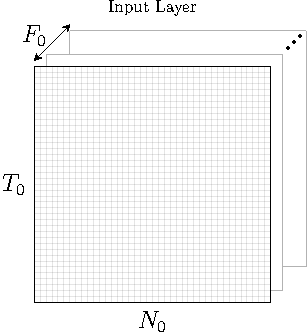
\includegraphics[scale=0.5]{input_layer}};
\end{tikzpicture}&=
%
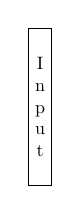
\begin{tikzpicture}[baseline=-0pt]
\draw (0,-1) rectangle (0+0.3,1);
\node[align=center,scale = 0.65] at (0+0.15,0) {I \\ n \\ p \\ u \\ t};
\end{tikzpicture}\;,&
%
\begin{tikzpicture}[baseline=-3pt]
\node[] at (0,0) {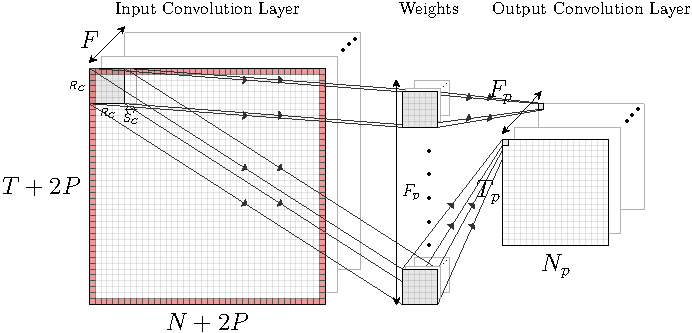
\includegraphics[scale=0.5]{VGG-conv}};
\end{tikzpicture}&=
%
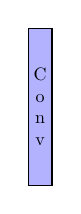
\begin{tikzpicture}[baseline=-0pt]
\filldraw[fill=blue!30!white] (0,-1) rectangle (0+0.3,1);
\node[align=center,scale = 0.65] at (0+0.15,0) {C \\ o \\ n \\ v};
\end{tikzpicture}\;,\notag\\
%
\begin{tikzpicture}[baseline=-3pt]
\node[] at (0,0) {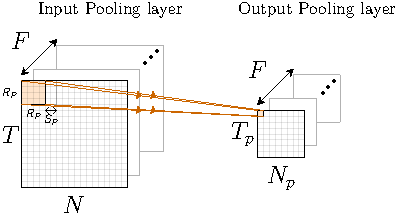
\includegraphics[scale=0.5]{VGG-pool}};
\end{tikzpicture}&=
%
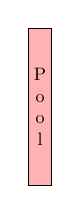
\begin{tikzpicture}[baseline=-0pt]
\filldraw[fill=red!30!white] (0,-1) rectangle (0+0.3,1);
\node[align=center,scale = 0.65] at (0+0.15,0) {P \\ o \\ o \\ l};
\end{tikzpicture}\;,&
%
\begin{tikzpicture}[baseline=-3pt]
\node[] at (0,0) {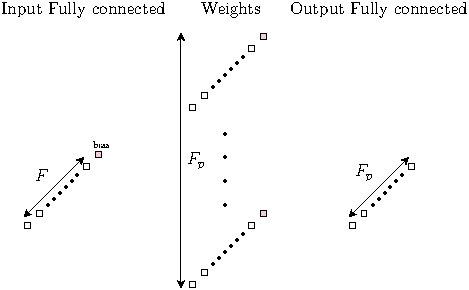
\includegraphics[scale=0.5]{VGG-fc}};
\end{tikzpicture}&=
%
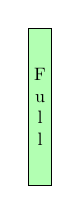
\begin{tikzpicture}[baseline=-0pt]
\filldraw[fill=green!30!white] (0,-1) rectangle (0+0.3,1);
\node[align=center,scale = 0.65] at (0+0.15,0) {F \\ u \\ l \\ l};
\end{tikzpicture}
\end{align*}
\begin{center}
\caption{CNN layers: Schematic representation}
\end{center}
\end{figure}

\newpara Based on these schematic layers, a simple graphical \footnote{\label{tomepel} Images source: Thomas Epelbaum GitHub: https:\textbackslash github.com\textbackslash tomepel \textbackslash Technical\_Book\_DLaccessed on 07th August 2019 } representation of VGG-Net is shown below.
\begin{figure}[t!]
\begin{center}
\begin{tikzpicture}
\node[] at (0,0) {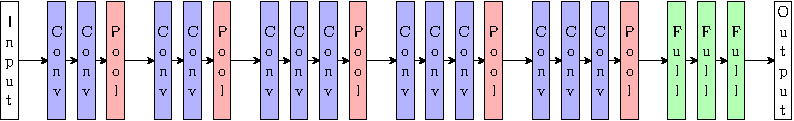
\includegraphics[scale=1]{VGG}};
\end{tikzpicture}
\caption{VGG-Net}
\end{center}
\end{figure} 
 
\section{RNN}
Recurrent neural network primarily are densely connected neural network simmilar to feed forward network with a key difference; introduction of \textit{time} component in RNN. The output of a hidden layer in an RNN is \textit{fed back } into itself. With this we can model the data which is time dependent or sequence dependent in nature. In programming terms this can be represented by a fixed program taking certain inputs and some internal variable.
\begin{center}

\begin{tikzpicture}[item/.style={circle,draw,thick,align=center},
itemc/.style={item,on chain,join}]
 \begin{scope}[start chain=going right,nodes=itemc,every
 join/.style={-latex,very thick},local bounding box=chain]
 \end{scope}
 \node[left=2em,item] (AL) {$A$};
 \path (AL.west) ++ (-1em,2em) coordinate (aux);
 \draw[very thick,-latex,rounded corners] (AL.east) -| ++ (1em,2em) -- (aux) 
 |- (AL.west);
 \draw[very thick,-latex] (AL.north) -- ++ (0,2em)
 node[above,item,fill=gray!10] {$h_t$};
 \draw[very thick,latex-] (AL.south) -- ++ (0,-2em)
 node[below,item,fill=gray!10] {$x_t$};
\end{tikzpicture}

\end{center}

\newpara The above diagram depicts a compact loop form of an RNN showing a loop. An RNN can be thought as a multiple copies of the same network, each previous network passing a message to it successor. By unrolling the compact for we can visualize the RNN as below. 

\begin{center}

\begin{tikzpicture}[item/.style={circle,draw,thick,align=center},
itemc/.style={item,on chain,join}]
 \begin{scope}[start chain=going right,nodes=itemc,every
 join/.style={-latex,very thick},local bounding box=chain]
 \path node (A0) {$A$} node (A1) {$A$} node (A2) {$A$} node[xshift=2em] (At)
 {$A$};
 \end{scope}
 \node[left=1em of chain,scale=2] (eq) {$=$};
 \node[left=2em of eq,item] (AL) {$A$};
 \path (AL.west) ++ (-1em,2em) coordinate (aux);
 \draw[very thick,-latex,rounded corners] (AL.east) -| ++ (1em,2em) -- (aux) 
 |- (AL.west);
 \foreach \X in {0,1,2,t} 
 {\draw[very thick,-latex] (A\X.north) -- ++ (0,2em)
 node[above,item,fill=gray!10] (h\X) {$h_\X$};
 \draw[very thick,latex-] (A\X.south) -- ++ (0,-2em)
 node[below,item,fill=gray!10] (x\X) {$x_\X$};}
 \draw[white,line width=0.8ex] (AL.north) -- ++ (0,1.9em);
 \draw[very thick,-latex] (AL.north) -- ++ (0,2em)
 node[above,item,fill=gray!10] {$h_t$};
 \draw[very thick,latex-] (AL.south) -- ++ (0,-2em)
 node[below,item,fill=gray!10] {$x_t$};
 \path (x2) -- (xt) node[midway,scale=2,font=\bfseries] {\dots};
\end{tikzpicture}
\end{center}

Mathematically RNNs can be represented as below: 

\begin{equation}
	\textbf{h}_t = f_W(\textbf{h}_{t-1} + \textbf{x}_{t}) 
\end{equation}

Where \textbf{\textit{ f}} is some function with parameter \textbf{W}. \\
This same function \textbf{\textit{ f}} and same weight matrix \textbf{W} is used at every step of the computation. \\
\textit{$h_t$} is new state \\
\textit{$h_{t-1}$} is old state \\
\textit{$x_t$} input vector at time step \textit{t}\\

In a more simplified form we can have the above function as:

\begin{equation}\label{hidden_state}
	\textbf{h}_t = \sigma (\textbf{Ux}_t + \textbf{Vh}_{t-1}) 
\end{equation}

Where \textit{U} is the input weight matrix and \textit{V} is the recurrent outputs. Time stamp denoted by \textit{t}. $\sigma$ represent an activation function e.g a \textit{tanh} or \textit{sigmoid}. If we unfold the above equation and go back three time step we have,

\begin{equation}
	\textbf{h}_t = \sigma (\textbf{Ux}_t + \textbf{V}(\sigma(\textbf{Ux}_{t-1} + \textbf{V}(\sigma(\textbf{Ux}_{t-2})))
\end{equation}

And in general, if we unfold in n time slot back,

\begin{equation}
\textbf{h}_t = \sigma (\textbf{Ux}_t + ...( \textbf{V}(\sigma(\textbf{Ux}_{t-n+2} + \textbf{V}(\sigma(\textbf{Ux}_{t-n+1})..)))
\end{equation}

\begin{equation}
	\textbf{y}_t = (\textbf{W}_{hy}  \textbf{h}_{t}) 
\end{equation}

Where \textbf{$y_t$}  represents output at a time stamp \textit{t} \\
\textbf{$h_t$} is the hidden state, computed as in equation \ref{hidden_state}

The problem in general suffered by a plain RNN is over a large period of time the back propagation gradients either exploding or vanishing. During a \textit{vanishing gradient } problem, the gradients of the network output with respect to the early layer of the network becomes extremely small, which indicates a large change in the parameters for the early layers does not have a big effect on network output. Usually this happens when the activation function such as \textit{sigmoid} or \textit{tanh} squash their input into a small output range non-linearly. Considering the activation function sigmoid which is defined as below,

\begin{equation}
	S(x) = \frac{1}{ 1+ e^x}
\end{equation}

Sigmoid is a special case of standard Logistic function defined as 
\begin{equation}
f(x) = \frac{L}{ 1+ e^{-k(x-x_0)}}
\end{equation}
Where \\
L: Curve's maximum value \\
k: Steepness of the curve \\
(x0 - x): value of Sigmoid's midpoint \\

A standard logistic function is called sigmoid when (k=1,x0=0,L=1) and can be viewed as below: \\

\begin{center}
\begin{tikzpicture}
	\begin{axis}%
		[
		grid=major,     
		xmin=-10,
		xmax=10,
		axis x line=bottom,
		ytick={0,.5,1},
		ymax=1,
		axis y line=middle,
		]
		\addplot%
		[
		blue,%
		mark=none,
		samples=200,
		domain=-6:6,
		]
		(x,{1/(1+exp(-x))});
	\end{axis}
\end{tikzpicture}

\end{center}
Sigmoid function can be re written as  \\
\begin{equation}
	S(x) = (1+e^{-x})^{-1}
\end{equation}
And by taking the derivative \\
\begin{equation}
\frac{d}{dx}S(x) = \frac{d}{dx} (1+e^{-x})^{-1} \\
= \frac{e^{-x}} {(1+e^{-x})^{-2}} 
\end{equation}

Plotting the derivative of the sigmoid activation function as below, we notice that 
\begin{center}

\begin{tikzpicture}
\begin{axis}%
[
grid=major,     
xmin=-10,
xmax=10,
axis x line=bottom,
ytick={0,.5,1},
ymax=1,
axis y line=middle,
]
\addplot%
[
blue,%
mark=none,
samples=100,
domain=-10:10,
]
(x,{exp(-x)/((1+exp(-x)) * (1+exp(-x)))});
\end{axis}
\end{tikzpicture}
\end{center}

the sigmoid derivative is well below the 1.0 in the whole range of input values. And this makes the gradients vanishing quite fast as, multiplying this value \footnote{value less than 1} several times for several layer \textit{ back propagation} brings the value close to 0.



\subsection{Models based RNN }
\newpara Abu Farha and team presented \cite{abu2018will} a similar work, where they discussed methods to predicts action that are considerably in future and their duration. And they tried to anticipate all activities within a horizon of 5 minutes. After inferring the activities from the observed part of the video using an RNN-HMM \cite{richard2017weakly}, they proposed two approaches to predict the future actions and their durations, in the first approach they used RNN, where the anticipated activities are fed to the RNN to predict the remaining duration of the on going activities and duration of the next activity along with its class.
In the second approach the proposed CNN based single pass model which predicts length and label of the future action. They have found that these both approach have outperformed both grammar based baseline and nearest neighbor baseline. RNN and CNN found to be performing similarly for time horizon more than 40 seconds and RNN performs better for lesser than 20 seconds time horizon. The task is more formally defined as,
given the first t frames $X_{\text{1}}^t$ \\
predict \[ C_{t+1}^T  = \ (C_{t+1}, ..., C_{T}) \]
where $C_{\text{i}}$ denotes action labels for unobserved frames
and the video is given by
\[ X_{1}^T = (X_{1}, ..., X_{T}) \]

\newpara
For the RNN training the loss function used as below
\begin{equation}
    L = -log\, \hat{p_c} + (l_r - \hat{l_r})^2 +  I (l_n - \hat{l_n})^2 
\end{equation}
where \\
$\hat{l_r}$ represents predicted remaining length of the current action, \\
$\hat{l_n}$ represents predicted length of the next action, \\
$\hat{p_c}$ is the predicted class of the next action

\newpara Unlike recursive strategy in RNN, CNN approach does the prediction in a one single pass.
Training data generated by using first 10\%, 20\%, 30\%, 50\% of the video as the observation and the following 50\% as the ground truth. During the training of the network squared error used as loss function.
\begin{equation}
    L = \frac{1} {SC} \sum_{a,c} (Y_{sc} - \hat{Y_{sc}})^2 
\end{equation}
where $\hat{Y}$ is the prediction of the network. \\
C represents action classes and \\
S number of rows for an action segment

\newpara Row-wise $\textit{l}_2$-normalization \footnote{$l_2$-norm of a real vector $x=(x_1,x_2,x_3)$ is given by $|x|=sqrt(x_1^2+x_2^2+x_3^2)$} of the output found to be more robust than softmax output with cross-entropy loss. \cite{abu2018will} did not elaborate the 'input sequence always end 1 second before the next action segment start'. What is the purpose of this and results if the input sequence is provided till the next action segment starts.

\newpara For the task of early detection, the goal is to recognize the activity with least possible amount of input observation \cite{ryoo2011human}. In \cite{ryoo2011human} they modeled the feature distribution over the course of observation by integral histogram representation of activities, and named the prediction algorithm as \textit{dynamic bag-of-words} as the prediction algorithm considers the sequential structure formed by video features. And they formulated the activity prediction process probabilistically as:
%\hat{f}(x,y) = \underset{(s,t)\in S_{xy}}{\mathrm{median}} \{g(s,t)\}
%\begin{equation}
%\begin{multlined}
\begin{align}
\begin{split}
	%\displaystyle \sum_{n=1}^\infty
		P(A_{p}\: |\: O,t) ={}& \displaystyle \sum_{d}  P(A_{p},d\: |\: O,t)\\
		={}&	\frac{\sum_{d} P(O\: | \: A_{p},d)P(t\: | \:d)P(A_{p},\: d)}
	 {\sum_{i}\sum_{d} P(O\: | \: A_{i},d)P(t\: | \:d)P(A_{i},\: d) }
\end{split}
\end{align}
%\end{multlined}
%\end{equation}

\newpara Where \textit{d} is a progress level of the activity \\
\textit{$A_{p}$}  \textit{ P(t|d)} represents the similarity between the observation length \textit{t} and that of the activity progress \textit{d}
\textit{P(O|Ap, d)} measures the similarity between the video observation and the activity \textit{$A_{p}$} with progress level \textit{d}. This \textit{integral bag-of-words} uses 3-D space-time local features and detect motion changes in the video and generates descriptors representing local movements in the video. These are cuboid feature descriptors \cite{dollar2005behavior}. After the features are extracted, \textit{k-means} clustering was applied and the clusters are knows as visual words. Every feature detected is now belong to one of this k-visual words. Then the activities are model as an integral histogram of visual-words. The similarity between a video and activity model was done by comparing their histogram representation. And finally dynamic programming was used to predict the ongoing activities from videos.

\section{LSTM Introduction}
\subsection{Models based on LSTM }




